

\chapter{Úvod}





\chapter{Java Enterprise edition 6}
V posledných rokoch prevláda tendencia tvorby komplexných systémov, ktoré spracovávajú veľké množstvá dát.
 


Java Enterprise Edition 6(Java EE 6) predstavuje platformu určenú na vývoj webových a podnikových aplikácií.\cite{fitWeb}Tieto aplikácie sú viacvrstvové z dôvodu lepšej prenositeľnosti,nasaditeľnosti a modifikovateľnosti. Frontend, predstavujúci užívateľské rozhranie a logiku na jeho ovládanie, pozostáva z webových frameworkov, stredná vrsta poskytuje bezpečnosť a transakcie. Najnižšia vrstva poskytuje pripojenie k databázam. Java EE 6 je vhodná pre implementáciu podnikovej logiky, ktorá dokáže byť riadená alebo interagovať s inými podnikovými aplikáciami. Java Enterprise Edition 6 je platformou, ktorá poskytuje širokú škálu aplikačných programových rozhraní(API), ktoré zjednodušujú, zkracujú a znižujú komplexnosť výslednej aplikácie. Jej vývoj neustále napreduje a je spravovaný Java Comunnity process(JCP).


\indent Java EE 6 bola uvoľnená v decembri 2009 a poskytuje ľahké používanie a kompletnú sadu nástrojov na tvorbu podnikových aplikácií. V súčastnosti vyšla ďalšia verzia, ktorá priniesla ďalšie novinky, ktoré môžte dohľadať v online dokumentácií. V ďalších kapitolách si rozoberieme aplikaný model jazyka, ktoré je veľmi dôležitý pre pochopenie princípu činnosti aplikácií vyvinutých touto platformou. Následne sa zameriame na JBoss a OptaPlanner, pre ktoré je určené užívateľské rozhranie. 


\section{Aplikačný model}
Java EE je určená pre implementáciu služieb pre zákazníkov, zamestnancov, dodávateľov kohokoľvek, kto prispieva do podniku. Takéto aplikácie sú komplexné a môže byť k nim pristupované z rozličných zdrojov. Pre lepšie zvládanie sú sústredené do stupňov.

\indent Java EE definuje spôsob implementácie služieb, ktoré sú škálovateľné, prístupné a spravovateľné podnikovou aplikáciou. Tento model implementuje viacstupňový model do nasledujúcich častí:
\begin{itemize}
\item Podniková a prezentačná logika poskytovaná Java EE platformou
\item Štandardná systémová platforma 
\end{itemize}

\section{Distribuovaná viacstupňová aplikácia}
Java EE používa aplikácie, ktoré sú viacvrstvové(multitier). Aplikačná logika je rozdelená medzi komponenty podľa funkcie.\cite{Pravidla} Jednotlivé komponenty sa následne rôzne inštalujú v závislosti, do ktorého stupňa patria. Jednotlivé stupňe sa skladajú z rôznych komponent:
\begin{itemize}
\item Klientská komponenta, ktorá beží na klientskom počítači
\item Webová komponenta, ktorá beží na Java EE serveri
\item Podniková komponentna, ktorá beží na Java EE serveri
\item Enterprise Information System software bežiaci na EIS serveri
\end{itemize}

Napriek tomúto rozloženiu býva aplikácia rozložená len do 3 stupňov: Java EE server, klient, databázy na pozadí. Typicky beží medzi klientskom a databázou častou viac-vláknový Java EE server, ktorý býva označovaný skratkou EIS. Viacstupňovérozloženie môžete názorne vidieť na obrázku č. \ref{model}.
\begin{figure}[htb]

\begin{center}

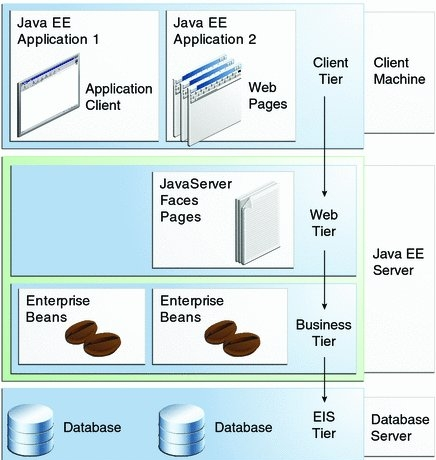
\includegraphics[scale=0.5]{model.jpg} 
\caption{Model Java EE, prevzaté z  http://docs.oracle.com/javaee/6/tutorial/doc/}
\label{model}

\end{center}

\end{figure}
Java EE aplikácia beží na klientskej stanici, býva obykle reprezentovaná tenkým klientom(webovým prehliadačom), nazývaným \uv{thin client}, alebo hrubým klientom, do ktoré je vložená logika aplikácia. V strednej časti obrázku sa nachádza Java EE server, na ktorom môžu bežať rôzne technológie v závislosti od požiadavky výslednej aplikácie. Java EE server môže by reprezentovaný rôznymi dostupnými technológiami, či už sa jedná o open-source riešenia (JBoss, Tomcat, GlassFish) alebo komerčné riešenia (IBM WebSphere,BEA WebLogic), ten obsahuje rôzne komponenty, ktoré so sebou rôzne komunikujú a interaugujú na požiadavky klienta a na druhej strane komunikujú s databázovým systémom. Tieto komponenty predstavujú logiku aplikáciu. Posledná časť predstavuje databázový systém, ktorý obsahuju dáta, ktoré klient požaduje pri svojom požiadavku, tento server sa nazýva "EIS" 
\newpage
\section{Bezpečnosť}

Java EE  vytvára prostriedky, ktoré sú prenositeľné a tak je možné systémy nasadzovať naprieč rôznymi platformami. Poskytuje mechanizmus  prístupovej kontroly pravidiel, ktoré sú interpretované, keď je aplikácia nasadzovaná na server. Java implementuje mechanizmus prihlasovania štandardne, čím odpadá programátori povinnosti túto časť dodatočne implementovať.

V ďalšej časti sa zameriame na podrobné vysvetlenie jednotlivých Java EE komponent, pretože ich pochopenie bude nevyhnuté.
\chapter{Java EE komponenty}
Java EE pozostáva z komponent, čo je vlastne sada sebestačného softwaru, ktorý je zhromaždený do Java EE aplikácií a komunikujú s inými komponentami. Java EE definuje nasledujúce komponenty: 
\begin{itemize}
\item Aplikačný klienti a aplety bežiaci na klientovi
\item Java Servlet, JavaServer Faces, and JavaServer Pages (JSP) komponenty bežia na Java EE serveri\cite{fitWeb}.
\item Enterprise JavaBeans (EJB) komponenty bežia na Java EE serveri\cite{fitWeb}.
\end{itemize}

V nasledujúcej časti sa zameriami na vysvetlenie jednotlivých pojmov, pretože sú doôležité z hľadiska pochopiteľnosti výslednej aplikácie.

\section{Java EE klienti}
Java EE client je typicky webový klient alebo aplikačný klient.

Typický webový klient pozostáva z dvoch častí:
\begin{itemize}
\item Dynamické webové stránky pozostávajúce z rôzneho značkovacieho jazyka(HTML, XML), ktoré sú generované webovými komponentami
\item Webovým prehliadačom, ktorý zobrazuje stránky
\end{itemize}
Typický webový klient sa nazýva "thin" klient, pretože nedotazuje nad databázou, alebo implementuje zložitú bussiness logiku. Všetky tieto činnosti vykonavá Java EE server. Klient len posiela požiadavky Java EE serveru a ten vykonáva dotazovanie a predávanie výsledkov.


Aplikační klienti bežia na klientských počítačoch, kde poskytujú bohatšie užívateľské rozhranie ako webový rozhrania značkovacích jazykov.
Typicky býva vytváraný technológiou Swing\footnote{http://cs.wikipedia.org/wiki/Swing\_(Java)} alebo Abstract Window Toolkit(AWT)\footnote{http://en.wikipedia.org/wiki/Abstract\_Window\_Toolkit}, občas sa vyskytuje aj prikázový riadok ako rozhranie.

\section{The JavaBeans Component Architecture}
Server a klient tiež zahŕňa komponenty založené na JavaBeans component architecture(JavaBeans components)\footnote{http://docs.oracle.com/javaee/1.4/tutorial/doc/JSPIntro8.html}, ktoré správujú toky dát medzi:
\begin{itemize}
\item Aplikačným klientom,alebo apletom a komponentami bežiacimi na Java EE serveri
\item Serverovými komponentami a databázami
\end{itemize}


Komunikácia medzi klientom s podnikovým stupňom, ktorý sa nachádza na Java EE serveri, v prípade, že klient beží v prehliadači.

\section{Webové komponenty}
Java EE webové komponenty sú súčasťou servletov alebo webových stránok, ktoré sú vytvorené JavaServer Faces technológiu\footnote{http://cs.wikipedia.org/wiki/JavaServer\_Faces}(JSF) and JavaServer pages(JSP)\footnote{http://cs.wikipedia.org/wiki/JavaServer\_Pages} technológiou.
Servlety sú javovské triedy , ktoré dynamicky spracovávajú požiadavky a tvoria odpovede. JSP stránky sú textové dokumenty, ktoré pracúvajú ako servlety ale umožňujú prirodzenejší prístup k vytváraniu statického obsahu. JavaServer Faces technológia stavia na servlety a JSP technológie a poskytuje užívateľské rozhranie komponentný framework pre webové aplikácie.


\subsection{Web Services}
Webové služby sú klientske a serverové aplikácie, ktoré komunikujú cez Hypertext Transfer Protocol (HTTP)\footnote{http://cs.wikipedia.org/wiki/Hypertext\_Transfer\_Protocol}. Webové služby poskytujú štandardné prostriedky, ktoré sú interoperabilné medzi softvérovými aplikáciami bežiacich na rôznych platformách. Webové služby sa vyznačujú veľkou interoperabilitou a rozšíriteľnosťou, rovnako ako ich strojovým spracovaním, vďaka použitiu XML. Webové služby môžu byť kombinované vo voľne spojených spôsoboch, ako dosiahnuť zložité operácie. Programy poskytujúce jednoduché služby môžu na seba vzájomne a poskytovať sofistikované služby.

\section{JavaServer Faces}
JavaServer Faces zodpovedá serverovej strane frameworku pre užívatelské rozhrania vychádzajúce z Javy. JavaServer Faces(JSF) vytvára aplikácie na základe MVC - Model-View Controller\footnote{http://en.wikipedia.org/wiki/Model-view-controller}. Ďalej treba spomenúť, že pomáha previazať užívatelské údaje so serverom, rovnako ako aj komponenty, ktoré sú znova použitelné.

\indent Aplikácia, ktorá je vytvára týmto frameworkom pozostáva z webových stránok, grafických komponent, sadou komponent naviazané na serverovú časť. Môže obsahovať rôzne desktriptory a konfiguračné súbory, ktoré nám pomáhujú pri nasadzovaní aplikácie. Základom JavaServer Faces je Facelets, čo je vlastne výzorovo deklaračný jazyk pre JSF. Facelets stránky používajú XHTML 1 a CSS\footnote{http://en.wikipedia.org/wiki/Cascading\_Style\_Sheets}. 

\section{Enterprise JavaBeans}
Enterprise JavaBeans(EJB) je používaný na vývoj a nasadzovanie komponentne založených aplikácií, ktoré sú škálovatelné a zabezpečené. Typicky obsahuje podnikovú logiku, ktorá pracuje s podnikovou databázou. Informácie o transakčných a bezpečnostných atribútoch býva typicky uložená v metadátach alebo v samostatnom XML súbore. Inštancia sa typicky spravuje za behu kontajnerom. Tento kontajner je prístupný klientovi. JavaBeans poskytuje všetky postriedky, ktorý súvisia s transakciami stavovým spravovaním, takže ponúkajú možnosť sa sústrediť na podnikovú logiku. 

V ďalšej časti sa zameriame na JBoss a OptaPlanner.

\section{Web Service}
Web Service je sú klientské a serverové aplikácie, ktoré komunikujú prostredníctvom HTTP protokolu vymenieňaním XML správ. Tieto aplikácie poskystujú interoperabilitu medzi rôznymi platformami naprieč počítačou sieťou. Web Service umožňuje komunikáciu medzi rôznymi aplikáciami, ktoré bežia na rôznych platformách, napr. Java aplikácie založené na Windowse komunikujú s Net. aplikácia bežiaci na Linuxe. Webo services  sa delia na 2 kategórie "big" web services a "RESTFul" web services.

\subsection{"Big" Web Services}
V Jave EE 6 existuje API, ktoré sa nazýva JAX-WS, ktoré umožňuje vytvorenie práve tohto typu web servici.\cite{fitWeb} "Big" web service využíva XML správy, spolu so SOAP a XML jazykom, ktorý definuje architekrúru a formát správ. Tento typ Web Service obsahuje definíciu pre Web Service vo formáte WSDL, ktorý je čitatelný aj počítačom. Formát SOAP správ a definíciu jazyka WSDL rozhrania môže znížiť zložitosť vývoja aplikácií, webových služieb. Design založený na SOAP musí obsahovať:
\begin{itemize}


\item    Musí byť stanovený formálný kontrakt pre popis rozhrania, ktoré web service ponúka . WSDL môže byť používaný na popis detailov, ktoré môžu zahŕňať správy, operácie, viazanie a umiestnenie webovej služby. 

\item    Architektúra musí riešiť zložité nefunkčné požiadavky. Mnoho špecifikácií web servicemusia riešiť takéto požiadavky a vytvoriť spoločný slovník pre nich. Príklady zahŕňajú transakcie , zabezpečenia, riešenie atď. .

\item    Architektúra musí zvládnuť asynchrónne spracovanie a vyvolanie  V takých prípadoch, infraštruktúra poskytuje štandardy , ako sú Web Services Reliable Messaging ( WSRM ) ,a API napr. JAX - WS.

\end{itemize}


\subsection{RESTful Web Service}
V Java EE 6 existuje pre druhý typ web service API, ktoré sa nazýva JAX - RS. Tento typ web serrvice je vhodný pre základné , ad hoc integračné scenáre. REST webové služby, často lepšie integrované s HTTP ako službami založenými na SOAP je , nevyžadujú XML správ alebo definície WSDL služby - API.

Tento typ web service je vhodný pokiaľ sú splnené nasledujúce kritéria:
\begin{itemize}
  \item  Web service sú bezstatové a potrebné zvážiť, či interakcia môže prežiť reštart servera .

  \item Využitie cache, pre dáta ktorá vracia web service nie je dynamicky generované a možno ich uložiť do vyrovnávacej pamäte , medzipamäte infraštruktúry , ktoré webové servery. O použitie sa musí postaráť programátor, pretože tieto cache sú obmedzené metódou HTTP GET.

   \item   Výrobca služby a služby pre spotrebiteľov majú vzájomné porozumenie kontextu a obsahu  ktorý je odovzdaný spolu. Neexistuje žiadny formálny spôsob, ako opísať rozhranie webových služieb, musie strany sa dorozumieť ako si budú vymieňať správy a čím aj správne rozumejú.

  \item  Web service alebo agregáciu do existujúcich webových stránok môže byť povolená ľahko pokojný štýl . Vývojári môžu používať také technológie ako JAX - RS a Asynchronous JavaScript s XML ( AJAX ) a také sady nástrojov , ako Direct Web Remoting ( DWR ) konzumovať služby vo svojich webových aplikáciách . Skôr než začínať od nuly , služby môžu byť vystavené s XML a spotrebované HTML stránok , bez toho, aby výrazne refactoring existujúce webové stránky architektúry . Existujúce vývojári budú viac produktívne , pretože sa pridá k niečomu , že sú už oboznámení s tým , skôr než by ste museli začať od nuly s novou technológiou.


\end{itemize}
\chapter{JBoss Aplication Server} 
JBoss, čo je vlastne skratka pre JavaBeans Open Source Applicatom Server, v súčastní nazývaný WildFly je aplikačný server, ktorý je založený na platforme Java a Java Enterprise Edition.\cite{jbossbook} Aplikačný server tvorí vrstvu medzi aplikáciami a operačným systémom, pričom rovnako poskytuje aplikácia často využívané funkcie, napr. spracovanie transakcií, výmená správ, atď. . Aplikačné servery podobne ako JBoss Aplication Server(JBoss AS) je open source. JBoss AS je od verzie 5 postavený na JBoss Microcontaineru(JBoss MC), čo je vlastne jadro, ktoré registruje služby(managed beans). Takto pre správu služieb tento server implementuje Java Management Extension(JMX).

 JBoss AS je napísaný v Jave, preto existuje možnosť  ho používať naprieč rôznym platformám. Tento server slúži na vývoj a nasadzovanie podnikových aplikácií, webových aplikácií, služieb a portálov. Tento server je licensovaný pod GNU Lesser General Public License(GNU PL).

\section{História JBoos-u}
Všetko naštartoval v roku 1999 Marc Fleury. Pre podporu vývoja middleware InterBohemia sebe rozhodol implementovať jeden zo štandardov J2EE , EJB kontajner. Tým sa zrodil prvý projekt - EJBoss, ktorý sa neskôr premenoval na JBoss. TO niekoľko rokov neskôr sa stal prvým certifikovaným  J2EE  open source aplikačným serverom. Ďalej by som rád ukázal na vývoj rôznych verzií JBossu:\cite{jbossWeb}


\begin{itemize}
\item JBoss AS 4.0 , Java EE aplikačný server 1.4 , je vybavený vloženým Apache Tomcat 5.5 servlet kontajnerom. JBoss môže bežať na mnohých operačných systémoch , vrátane mnohých POSIX platformách (ako GNU/Linux , FreeBSD a Mac OS X) , Microsoft Windows a ďalšie,.
\item JBoss AS 5.1 , povolený v roku 2009 , pracuje ako Java EE 5 aplikačný server. Je to menšia aktualizácia hlavnej verzie JBoss AS 5.0, ktorý bol vo vývoji po dobu najmenej troch rokov a bol postavený na vrchole novej JBoss microcontainer.

\item JBoss AS 6.0 , bol neoficiálne implementáciou Java EE 6 , vydané 28. decembra 2010 .

\item JBoss AS 7 , bola vydané 12. júla 2011 , len šesť mesiacov po poslednej hlavnej verzie , JBoss AS 6. JBoss AS 7 podporuje rovnaké špecifikáciu Java EE ako posledná verzia, a to Java EE 6. Java EE profil je iba čiastočne implementovaný v JBoss AS 7. Hlavné zmeny viditeľné pre užívateľa sú : oveľa menšiu veľkosť ( menej než polovica z JBoss AS 6 ) a násobné zníženie v čase spustenia.

\item JBoss AS 7.1 , aktuálna stabilná verzia bola vydaná vo februári 2012 . Zostávajúce časti EE špecifikácie boli realizované , a táto verzia bola certifikovaná pre EE plnom profile.

\item WildFly 8 je priamym pokračovaním na JBoss AS projektu .

\end{itemize}

V ďalšej časti sa zameriame na OptaPlanner\footnote{http://www.optaplanner.org/}, čo je vlastne systém, pre ktorý je rozhranie navrhované.




\section{OptaPlanner}
 Optaplanner je framework, kde si môžete vytvoriť pravidlá, ktoré určujú, kedy by mali byť vykonané špecifické akcie. To by mohlo byť vykonané v kóde za použitia podmienok.
OptaPlanner je odĺahčený open source software a ďalšie prokračovanie frameworku JBoss Drools, ktoré optimalizuje plánovacie problémy.\cite{optaweb} Tieto plánovacie problémy môžu byť nasledujúceho charakteru: 
\begin{itemize}
\item Plánovanie agendy: plánovanie schôdzok, vymenovanie, práca údržby, reklama, ...
\item Plánovanie vzdelávania: plánovanie lekcie, kurzov, skúškov, prezentácie na konferenciách, ...
\end{itemize}
\begin{figure}[htb]

\begin{center}

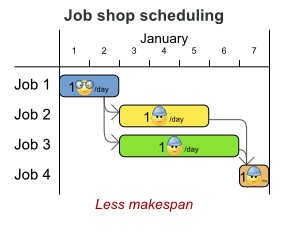
\includegraphics[scale=0.5]{fig/useCaseOverview.jpg} 
\caption{Job  Shop scheluding, prevzaté z  }
\label{obrazokUseCase}

\end{center}

\end{figure}
Obrázok č. \ref{obrazokUseCase} zobrazuje typické použitie OptaPlanner-u. Môžme vidieť v nasledujúcom obrázku vystupú 4 osoby, ktoré vykonávajú nejakú činnosť. Ich činnosť je špecifická a silne závisí od práce predchádzajúcich. Optaplanner sa snaží ich činnosti maximálne optimalizovať a jednotlivé činnosti zvoliť v následnosti tak, aby výsledná práca bola spravená za najkratší možný čas vzhľadom na činnosť, ktorá sa optimalizuje.


OptaPlanner pomáha Java programátorom riešiť  constraint satisfaction efektívne.

\subsection{NP-úplný problém}
Každý plánovací problém je NP-úplný problém.\cite{npbook} NP-úplné problémy sú nedeterministicky polynomiálne problémny, na ktoré sú redukovateľné všetky ostatné NP problémy. Tieto problémy nie sú riešitelné v dostupnom čase, pretože sa nepodarilo nájsť deterministický algoritmus. Príkladom NP úloh môžme považovať: problém obchodné cestujúceho, hľadanie nezávislej množiny, atď. . 

Riešenia poskytnutým týmto frameworkom, ktorý využíva pokročilé optimalizačné algoritmy, sú dosiahnuteľné v reálnom čase. Dosiahnutie v reálnom čase znamená nájdenie 1 alebo viacerých riešení, alebo nenájdenie žiadneho riešenia vzhľadom na poskytnutý čas a optimalizačné algoritmy.

Každý plánovací rpbolém je definovaný na základe obmedzení, ktoré musia minimálne spĺnať: \cite{optabook}
\begin{itemize}
\item Negatívne "hard" obmedzenie, ktoré nesmie byť porušené
\item Negatívne "soft" obmedzenie, ktoré by nemali byť porušené pokiaľ sa dá tomu vyhnúť.
\end{itemize}

Niektoré problémy môžu obsahovať aj pozitívne podmienky alebo odmeny, ktoré by mali byť splnené pokiaľ je možné ich splniť.

Tieto podmienky definujú skóre kalkuláciu plánovacieho problému. Tieto podmienky môžu byť zapísané v Jave alebo v Drools pravidlách, ktoré značne zjednodušujú kód.




 Vytvorenie je pomocou pravidiel  môže robiť  oveľa jednoduchšie spájať mnoho pravidiel s mnohými akciami. Tieto pravidlá bývajú typicky definované pomocou XML súboru.

OptaPlanner pomáha  programátori riešiť obmedzenie problémov spokojnosti efektívne. Pod kapotou sa kombinuje optimalizačné heuristiky na výpočet skóre.






\subsection{Výsledky plánovacieho problému}

Tieto obmedzenia definujú výpočetné skóre problému plánovania. Každé riešenie problému plánovanie môže byť odstupňovaná so skóre. 

Plánovanie problému má niekoľko riešení . Existuje niekoľko kategórií riešení:
\begin{itemize}
\item Možným riešením je nejaké riešenie, či je alebo nie je ľubovoľný počet obmedzení. Problémy plánovanie mávajú neuveriteľne veľké množstvo možných riešení. Mnoho z týchto riešení sú bezcenné .
\item Uskutočniteľným riešením je riešenie, ktoré neporušuje žiadne (negatívne) tvrdé obmedzenia. Niekedy nie sú realizovateľné riešenie. Každý uskutočniteľné riešenie je možné riešenie.

\item Optimálnym riešením je riešenie s najvyšším počtom bodov . Problémy plánovanie mávajú jedno alebo niekoľko optimálnych riešení. K dispozícii je vždy aspoň 1 optimálnym riešením, a to aj v prípade , že neexistujú žiadne uskutočniteľné riešenie, a optimálne riešenie nie je možné .
\item Najlepším riešením je nájsť riešenie s najvyšším skóre zistené implementáciou v danom čase.

\end{itemize}

OptaPlanner podporuje niekoľko optimalizačných algoritmov ako efektívne prehrýzť týmto neuveriteľne veľkým množstvom možných riešení. V závislosti na prípade použitia, niektoré optimalizačné algoritmy dosahujú lepšie výsledky ako ostatné, ale to je nemožné povedať dopredu. Pri plánovaní , je ľahké prepnúť algoritmus optimalizácie, zmenou konfigurácie Solver na niekoľkých riadkov XML alebo kódu.


\newpage
\subsection{Ukážka XML configuračného súboru}
V nasledujúcom obrázku by som rád ukázal príklad XML configuračného súboru pre OptaPlanner.
 \lstset{
    language=xml,
    tabsize=3,
    %frame=lines,
    caption=Test,
    label=code:sample,
    frame=shadowbox,
    rulesepcolor=\color{gray},
    xleftmargin=20pt,
    framexleftmargin=15pt,
    keywordstyle=\color{blue}\bf,
    commentstyle=\color{OliveGreen},
    stringstyle=\color{red},
    numbers=left,
    numberstyle=\tiny,
    numbersep=5pt,
    breaklines=true,
    showstringspaces=false,
    basicstyle=\footnotesize,
    emph={food,name,price},emphstyle={\color{magenta}}}
    \lstinputlisting{cloudBalancingSolverConfig.xml}

\newpage
Konfigurácie solveru pozostáva z 3 častí: 
\begin{itemize}
\item Domail model configuration: Musíme Optaplanneru uviesť hlávnú triedu.
\item Configurácia skóre, ktorá hovoŕí Optaplanneru ako ma optimalizova premenné. Pokiaľ používame hard a soft obmedzenia, pouźijeme "HardSoftScore". Musíme tiež povedať, Planner, ako vypočítať také skóre, v závislosti na našich obchodných požiadavok. Ďalej sa, sme musíme  pozrieť do 2 alternatívy pre výpočet skóre: pomocou jednoduchej implementácie Java, alebo pomocou Drols DRL.Plánovanie bude hľadať riešenie s najvyšším skóre. Budeme používať HardSoftScore, čo znamená, plánovač bude hľadať riešenie s žiadnymi tvrdými obmedzeniami členenie (spĺňajú požiadavky na hardvér) a pokiaľ možno čo najmenej mäkkých obmedzenia členenie (minimalizovať náklady na údržbu).
\item Konfigurácia Optimalizačné algoritmy: Ako by Plánovanie optimalizovať? Nebojte sa o tom teraz: je to dobrý východiskový nastavenie, ktoré funguje na väčšine problémov, plánovanie. To sa už predčí ľudské plánovača a väčšina in-house implementáciou. Použitie Planner porovnávacie toolkit, môžete vyladiť, aby to bolo ešte lepšie výsledky.

\end{itemize}

\subsection{Optimalizačné algoritmy}
\begin{itemize}
\item First FIT - To je veľmi jednoduché greedy algoritmus aproximácie. Algoritmus spracováva položky v ľubovoľnom poradí . Pre každú položku , pokúsi sa umiestniť na položku v prvom koši , ktorý sa môže ubytovať položku . Ak nie je nájdený žiadny bin , otvára novú priehradku a kladie položku v rámci nového zásobníka .

To je pomerne jednoduché zobrazenie tento algoritmus dosahuje aproximačnou faktor 2 , to znamená , že počet nádob , ktoré tento algoritmus je viac ako dvojnásobok optimálny počet zásobníkov . To je spôsobené tým , zistenie , že v danom čase , že je nemožné , 2 nádoby , aby sa maximálne polovice plná . Dôvodom je , že ak by to bolo možné , znamenalo by to , že v určitom okamihu presne jeden bin bol najviac polovicu plné a nový bol otvorený ubytovať položiek o veľkosti nanajvýš V / 2. Ale od tej doby prvý , kto má aspoň priestor V / 2 , algoritmus nebude otvárať nové kôš pre každú položku , ktorej veľkosť je nanajvýš V / 2. Až po bin naplní viac ako V / 2 alebo chcete položku s veľkosťou väčšou ako V / 2 dorazí , môže algoritmus otvoriť novú priehradku .

Ak teda máme koša B , aspoň B - 1 koše sú viac než z polovice plná .
\item Firt FIT Decreasing
\item Firt FIT Decreasing + heurestic local search(

\begin{itemize}
\item Hill Climbing -horolezectvo je matematická optimalizácia technika , ktorá patrí do rodiny miestneho vyhľadávania . Jedná sa o iteratívny algoritmus , ktorý začína s ľubovoľným riešenie problému, potom sa pokúsi nájsť lepšie riešenie tým , že postupne mení jeden prvok riešenia . Ak zmena vytvára lepšie riešenie , postupné zmeny je , aby nové riešenie , opakovať až do žiadne ďalšie zlepšenie možno nájsť .

Napríklad , horolezectvo môžu byť použité k problému obchodného cestujúceho . Je ľahké nájsť prvé riešenie , ktoré navštívi všetky miesta , ale bude veľmi zlá v porovnaní s optimálne riešenie . Algoritmus začína s takýmto riešením a robí drobné vylepšenia k nemu , ako napríklad prepínanie poradí , v ktorom sú navštívili dve mestá . Nakoniec , oveľa kratšia cesta je pravdepodobné , že bude získaný.

Hill lezenie je dobré pre nájdenie lokálneho optima ( riešenie , ktoré nemôže byť zlepšená tým , že zvažuje susedné konfiguráciu ) , ale nie je zaručené , že nájsť najlepšie možné riešenie (globálne optimálne ) zo všetkých možných riešení ( priestor hľadania ) . Charakteristické , že iba lokálne optima sú zaručené môže byť vyliečených pomocou reštartuje ( opakované miestne vyhľadávanie ) , alebo zložitejšie schémy na základe iterácií , ako iteratívny lokálne vyhľadávanie v pamäti , rovnako ako reaktívne optimalizácia pre vyhľadávače a Tabu prehľadávanie , alebo pamäť , menej náhodných zmien , rovnako ako simulované žíhanie . \cite{algobook}




\item Tabu Search - Tabu prehľadávanie používa miestnej alebo susedstve vyhľadávanie postup iteratívne presunúť z jedného možného riešenia x k lepšiemu riešeniu x  v susedstve x , kým sa niektorá zastavenie kritériom bol splnený ( Všeobecne platí , že obmedzenia pokus alebo prah skóre ) . Miestne postupy vyhľadávania sa často stávajú uviazol v zlej bodovania oblastiach alebo v oblastiach, kde skóre plošine . V snahe vyhnúť sa týmto nástrahám a preskúmať oblasti hľadaného miesta , ktorá by mala zostať bez prehliadky inými miestnymi postupmi vyhľadávanie , tabu search starostlivo skúma okolí každého roztoku ako hľadanie postupuje . Riešenie prijatí do novej štvrti , $N ^ * ( x )$ , sú určené pomocou pamäťových štruktúr . Pomocou týchto pamäťových štruktúr , 
F
Tieto pamäťové štruktúry tvorí to , čo je známe ako zoznam tabu , súborom pravidiel a zakázaných riešenie slúži na filtrovanie , ktoré riešenie bude prijatý do susedstva $N ^ * ( x )$ , ktoré majú byť skúmané vyhľadávanie . Vo svojej najjednoduchšej forme , zoznam tabu je krátkodobý sadu riešení , ktoré boli navštívené v nedávnej minulosti ( menej ako n iterácií pred , kde n je počet predchádzajúcich riešeniach , ktoré možno uložiť - je tiež nazývaný tabu držba ) . Všeobecnejšie , zoznam tabu sa skladá z riešení , ktoré boli zmenené v procese prechodu od jedného do druhého roztoku . Je vhodný pre ľahké popisu pochopiť " riešenie " , ktorý má byť kódovaný a predstavované týmito atribútmi .

\item Simulated Annealing - Simulované žíhanie ( SA ) je všeobecný pravdepodobnostné metaheuristic pre globálne optimalizačné problém lokalizovať dobré priblíženie k globálnej optimálnej danej funkcie vo veľkom vyhľadávacieho priestoru . To sa často používa pri hľadaní priestorov je diskrétne ( napr. všetky výlety , ktoré navštevujú danú množinu miest ) . U niektorých problémov , môže simulované žíhanie byť účinnejšie ako vyčerpávajúci zoznam - za predpokladu , že cieľom je iba nájsť prijateľne dobré riešenie v stanovenú dobu , skôr ako tým najlepším možným riešením .

Názov a inšpirácia pochádza z žíhanie v metalurgii , technika zahŕňajúce vykurovania a riadeného ochladzovania materiálu k zvýšeniu veľkosti svojich kryštálov a znížiť ich vady . Obaja sú vlastnosti materiálu , ktorý závisí na jeho termodynamickej voľnej energie . Vykurovanie a chladenie materiálu má vplyv na teplotu a termodynamickú voľnú energiu . Aj keď rovnaké množstvo chladenie prináša rovnaké množstvo poklesu teploty je prinesie väčší alebo menší pokles termodynamickej voľnej energie v závislosti na rýchlosti , ktorá sa vyskytuje , s pomalším tempom produkujúce väčší pokles .

Tento pojem pomalého ochladzovania sa vykonáva v simulované žíhanie algoritmu , ktorý je pomalý pokles v pravdepodobnosti prijatia horšie riešenie , ako sa zaoberá riešenie priestoru . Prijatie horšie riešenie je základná vlastnosť metaheuristics , pretože to umožňuje rozsiahlejšie hľadanie optimálneho riešenia .

Táto metóda bola nezávisle opísal Scott Kirkpatrick , C. Daniel Gelatt a Mario P. Vecchi v roku 1983 , [ 1 ] a Vlado Černý v roku 1985 . [ 2 ] Táto metóda je adaptáciou Metropolis - Hastings algoritmus , metóda Monte Carlo generovať vzorové stavy termodynamického systému , vynájdený MN Rosenbluth a publikované v dokumente N. Metropolis et al . v roku 1953 . [ 3 ]

\end{itemize}

\end{itemize}


V ďalšej kapitole by som rád uviedol problematiku užívateľského rozhrania.
\chapter{Grafické užívateľské rozhranie}
V tejto kapitole sa zameráme na problematiku užívateľského rozhrania, ktoré vlastne je reprezentované Web services. Toto rozhranie bude umožňovať nahrávať pravidlá, zobrazovať výsledky, spúšťať, pozastovať a zobrazovať detaily úloh. Keďže táto výsledná aplikácia by mala byť použíteľná aj na mobilnom telefóne bol vybratý štýlovací framework Twitter Bootstrap, ktorý značne uľahčenie tvorbu takéhoto rozhrania.

\section{Twitter Bootstrap}
Twitter Bootstrapje veľmi jednoduchý a voľne dostupný súbor nástrojov pre vytváranie moderného webu a webových aplikácií.\cite{boot} Ponúka podporu najrôznejších webových technológií HTML , CSS , JavaScript\footnote{http://en.wikipedia.org/wiki/Javascript} a mnoho prvkov , ktoré je možné ľahko implementovať do svojej stránky. Pre použitie Twitter Bootstrap sú nutné základné znalosti HTML a CSS. Interaktívne prvky ako sú tlačidlá, boxy , menu a ďalšie kompletne nastavené a graficky spracované elementy je možné vložiť iba pomocou HTML a CSS .

\subsection{História}
Mark Otto a Jacob Thornton z Twitteru vyvinuli Twitter Bootstrap ako framework pre podporu konzistencie interných nástrojov. Pred vyvinutím Twitter bootstrap , boli v spoločnosti používané rôzne knižnice pre vývoj rozhrania, čo viedlo k nejednotnosti zdrojových kódov a vysokým nákladom na údržbu.


\subsection{Výhody}
Výhodou tohto súboru nástrojov je jednoduché spracovanie akéhokoľvek používateľského rozhrania vo webovej aplikácii a nerozhoduje , či to je napríklad používateľské rozhranie v administrácii back-endových alebo front-endových aplikácií.

\subsection{Komponenty}
Dohromady poskytujú komponenty a JavaScript pluginy nasledujúce elementy užívateľského prostredia:
\begin{itemize}
\item Button groups - Skupiny tlačidiel
\item Button dropdowns - Vysúvacia tlačidla
\item Navigational tabs, pills, and lists - Záložky, pilulky a zoznamy pre navigáciu
\item Navbar - navigačné položky
\item Labels - štítky
\item Badges - "odznáčiky"
\item Page headers and hero unit - hlavičky stránky a "hero unit"
\item Thumbnails - náhľady
\item Alerts - výstrahy
\item progress bars
\item Modals
\item Dropdowns - vysúvacie menu
\item Tooltips
\item Popovers
\item Accordion
\item Carousel - posuvný slider
\item Typeahead
\end{itemize}

Podrobné vysvetlenie jednotlivých komponent nájdete na nasledujúcej adrese http://getbootstrap.com/, rovnako aj s príkladmi použitia. V nasledujúcej časti prejdem na samotný návrh užívateľského rozhrania.

\section{Návrh rozhrania}
Výsledné rozhranie kladie dôraz na jednoduchosť a prehľadnosť zobrazených úloh. Rozhranie je rozdelené na 2 časti. Prvá časť, obrázok č.\ref{nahratie} popisuje spôsob nahratia xml súboru zo súborového systému. Užívateľ stlačí tlačidlo na nahratie xml, kde sa následne zobrazí obsah súborového systému a užívateľ zvolí príslušný xml súbor. Následne sa vyplnia údaje o názve súboru a počtu pravidiel v xml. Následne užívateľ potvrdí výber tlačidom "OK" a prejde na hlavné okno,ktoré priebežne zobrazuje stav vykonávania úlohy a informácie o úlohe.
\begin{figure}[!htb]

\begin{center}

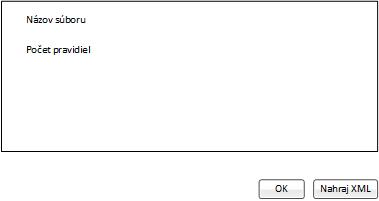
\includegraphics[scale=0.8]{NahratieSuboru.jpg} 
\caption{Ukážka nahratia súboru}
\label{nahratie}

\end{center}

\end{figure}

Ďalej by som rád ukázal na obrázku č. \ref{zobrazenie} spôsob zobrazovania úloh spolu s jeho stavom. Toho rozhranie sa dá rozdeliť na 2 časti: Prvá časť je reprezentovaná tlačidlami, ktoré reprezentujú spôsob na : 
\begin{itemize}
\item Pridávanie nových úloh, ktoré po stlačení zobrazí okno, ktoré je reprezentované obr. č. \ref{nahratie}
\item Editovanie skončenej úlohy
\item Zrušenie vybranej úlohy
\item Spravovanie užívateľov(platí pre rolu Administrátor)
\item Pozostavenie bežiacej úlohy

\end{itemize}

Ďalšia časť zobrazuje úlohy. Každá úloha je reprezentovaná rôznymi informáciami, ktoré sú rozdelé do stĺpcov. Každý záznam je prezentovaný položkou ID, ktorá reprezentuje jedinečný identifikátor v rámci systému spracovania, názvu úlohy, ktorá bola vyextrahovaná z xml súboru, statusu úlohy, ktoré je reprezentovaný 3 položkami:
\begin{itemize}
\item Dokončená úloha - finished
\item Running - bežiaca úloha
\item Paused - pozastavená úloha
\end{itemize}
, ukazateľom spracovania úloh, ktorá ukazuje aktuálne spracovania úlohy a položkou ETA, ktorá ukazuje odhadovaný čas do konca spracovania úlohy. Daná tabuľka obsahuje viacero položiek, ktoré rôzne zobrazujú stavy úloh. Úlohy v stave "finished" je možné otvoriť a zobraziť detaily spracovania, zmeniť parametre a spustiť nový beh úlohy, pričom pôvodná úloha zostane zachovaná. Pridávanie úloh možno realizovať aj za behu iných úloh, rovnako pozastavené úlohy možno znova spustiť z inými detailami.

\begin{figure}[h]

\begin{center}

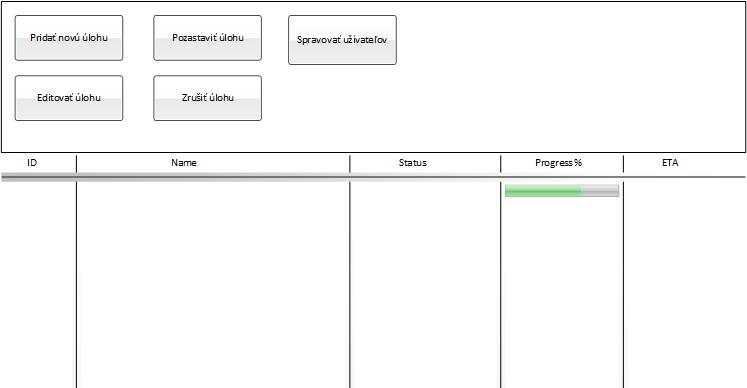
\includegraphics[scale=0.8]{Zobrazenie.jpg} 
\caption{Ukážka zobrazenie stavu úloh}
\label{zobrazenie}

\end{center}

\end{figure}





\chapter{Záver}
Táto práca je zameraná na priblíženie technológie Java EE 6, JBoss, OptaPlanner a výsledného rozhrania. Bežnému užívateľovi sú krok po kroku vysvetlované všetky používané metódy. Všetky tieto technológie sú voľne dostupné na internete, preto užívateľ má možnosť sa naučené veci vyskúšať si aj svojpomocne. Výsledný návrh rozhrania kladie dôraz na jednoduchosť, prehľadnosť a širokú podporu. Všetky tieto nové technológie mi pomohli zlepšiť rozhľad v IT technológiách a ukázali mne aj iným  princíp podnikových apikácií, ktoré sa dnes vyvíjajú a používajú.



